\documentclass{article}
\usepackage[utf8]{inputenc}
\usepackage{geometry}
\usepackage{enumitem}
\usepackage{hyperref}
\usepackage{xcolor}
\usepackage{graphicx}
\usepackage{array}
\usepackage{multirow}
\usepackage{amsmath, amssymb}
\usepackage{chemfig}
\usepackage{mhchem}
\usepackage{tikz}
\usepackage{setspace}
\usepackage{soul}
\usepackage{mathtools}
\usepackage{booktabs}
\usepackage{chemformula}
\usepackage{siunitx}
\usetikzlibrary{positioning, calc}
\usepackage{longtable}
\geometry{margin=1in}
\setlength{\parskip}{0.5em}
\usepackage{cancel}

\newcommand{\lewisdot}[5]{% #1=element, #2=initial dots, #3=arrow label, #4=final dots, #5=charge
\begin{tikzpicture}[node distance=1.2cm,baseline=(E.base)]
\node (E) {#1};
\foreach \pos in {#2} {\fill ($(E.center)+\pos$) circle (1.6pt);}
\node[right=0.8cm of E] (arrow) {\(\xrightarrow{#3}\)};
\node[right=1.6cm of E] {$[$};
\node[right=2.2cm of E] (Ei) {#1};
\foreach \pos in {#4} {\fill ($(Ei.center)+\pos$) circle (1.6pt);}
\node[right=0.4cm of Ei] {$]^{#5}$};
\end{tikzpicture}}

% Coordinate macros
\def\NaDot{(0.4,0)}
\def\Na2Dot{(0.35,0.05),(0.35,-0.05)}

\def\ClNeutral{(-0.05,0.4),(0.05,0.4),(-0.4,-0.05),(-0.4,0.05),(-0.05,-0.4),(0.05,-0.4),(0.4,0)}
\def\ClAnion{(-0.05,0.4),(0.05,0.4),(0.4,-0.05),(0.4,0.05),(-0.05,-0.4),(0.05,-0.4),(-0.4,-0.05),(-0.4,0.05)}
\def\ClCExtra{(0,0.4),(0.4,0),(0,-0.4),(-0.4,0),(0.3,0.3)}

\def\SDot{(-0.05,0.4),(0.05,0.4),(-0.4,-0.05),(-0.4,0.05),(0.4,0),(0,-0.4)}
\def\SAnion{(-0.05,0.4),(0.05,0.4),(0.4,-0.05),(0.4,0.05),(-0.05,-0.4),(0.05,-0.4),(-0.4,-0.05),(-0.4,0.05)}
\def\SCExtra{(0,0.4),(0.4,0),(0,-0.4),(-0.4,0),(0.3,0.3),(-0.3,-0.3),(0.3,-0.3),(-0.3,0.3)}

\def\MgDot{\Na2Dot}
\def\MgAnion{(0.4,0),(-0.4,0),(0,0.4),(0,-0.4)}

\def\CuDot{(0.4,0)}
\def\CuAnion{(0.4,0),(-0.4,0)}

\def\NDot{(-0.05,0.4),(0.05,0.4),(0.4,0),(0,-0.4),(-0.4,0)}
\def\NAnion{(-0.05,0.4),(0.05,0.4),(0.4,-0.05),(0.4,0.05),(-0.05,-0.4),(0.05,-0.4),(-0.4,-0.05),(-0.4,0.05)}
\def\NCExtra{(0,0.4),(0.4,0),(0,-0.4),(-0.4,0),(0.3,0.3),(-0.3,0.3),(0.3,-0.3),(-0.3,-0.3)}



\begin{document}

\begin{center}
    \vspace*{-1cm}
    \begin{tabular}{p{12cm} r}
        & \textbf{Name:} \underline{\hspace{5cm}} \\
    \end{tabular}

    \vspace{0.5cm}
    {\LARGE \textbf{Week 7 Worksheet}}
\end{center}    
\\

\vspace{0.5cm}
\noindent \begin{tabular}{|p{0.9\linewidth}|}
\hline
\vspace{0.2cm}
\textbf{(1)} Calculate the atomic mass of carbon given its common isotopes: $^{12}\text{C}$ has mass $12.000000$ amu (98.930\%) and $^{13}\text{C}$ has mass $13.003355$ amu (1.070\%). \\
\begin{minipage}[t]{0.85\linewidth}
\begin{enumerate}[label=\alph*.]
\item 12.001 amu
\item 12.01 amu
\item 12.10 amu
\item 13.003 amu
\end{enumerate}
\end{minipage}\\
\hline
\end{tabular}
\\

\vspace{0.5cm}
\noindent \begin{tabular}{|p{0.9\linewidth}|}
\hline
\vspace{0.2cm}
\textbf{(2)} Calculate the atomic mass of chlorine given its common isotopes: $^{35}\text{Cl}$ mass $=34.96885$ amu (75.78\%), $^{37}\text{Cl}$ mass $=36.96590$ amu (24.22\%). \\
\begin{minipage}[t]{0.85\linewidth}
\begin{enumerate}[label=\alph*.]
   \item 35.00 amu
   \item 35.178 amu
   \item 35.45 amu
   \item 36.000 amu
\end{enumerate}
\end{minipage}\\
\hline
\end{tabular}
\\

\vspace{0.5cm}
\noindent \begin{tabular}{|p{0.9\linewidth}|}
\hline
\vspace{0.2cm}
\textbf{(3)} Calculate the atomic mass of magnesium using three common isotopes: $^{24}\text{Mg}$ mass $=23.985042$ amu (78.99\%), $^{25}\text{Mg}$ mass $=24.985837$ amu (10.00\%), $^{26}\text{Mg}$ mass $=25.982593$ amu (11.01\%). \\
\begin{minipage}[t]{0.85\linewidth}
\begin{enumerate}[label=\alph*.]
   \item 24.31 amu
   \item 24.000 amu
   \item 25.000 amu
   \item 23.985 amu
\end{enumerate}
\end{minipage}\\
\hline
\end{tabular}
\\

\vspace{0.5cm}
\noindent \begin{tabular}{|p{0.9\linewidth}|}
\hline
\vspace{0.2cm}
\textbf{(4)} Calculate the atomic mass of silver from its two stable isotopes: $^{107}\text{Ag}$ mass $=106.90509$ amu (51.839\%), $^{109}\text{Ag}$ mass $=108.90476$ amu (48.161\%). \\
\begin{minipage}[t]{0.85\linewidth}
\begin{enumerate}[label=\alph*.]
   \item 107.000 amu
   \item 107.868 amu
   \item 108.000 amu
   \item 106.905 amu
\end{enumerate}
\end{minipage}\\
\hline
\end{tabular}
\\
 \newpage \noindent 
\noindent \begin{tabular}{|p{0.9\linewidth}|}
\hline
\vspace{0.2cm}
\textbf{(5)} Calculate the atomic mass of bromine given: $^{79}\text{Br}$ mass $=78.918337$ amu (50.690\%), $^{81}\text{Br}$ mass $=80.916291$ amu (49.310\%). \\
\begin{minipage}[t]{0.85\linewidth}
\begin{enumerate}[label=\alph*.]
   \item 79.000 amu
   \item 80.500 amu
   \item 79.903 amu
   \item 78.918 amu
\end{enumerate}
\end{minipage}\\
\hline
\end{tabular}
\\

\vspace{0.5cm}
\noindent \begin{tabular}{|p{0.9\linewidth}|}
\hline
\vspace{0.2cm}
\textbf{(6)} Which group of the periodic table do the alkali metals belong to? \\
\begin{minipage}[t]{0.85\linewidth}
\begin{enumerate}[label=\alph*.]
\item Group 1
\item Group 2
\item Group 17
\item Group 18
\end{enumerate}
\end{minipage}\\
\hline
\end{tabular}
\\

\vspace{0.5cm}
\noindent \begin{tabular}{|p{0.9\linewidth}|}
\hline
\vspace{0.2cm}
\textbf{(7)} Calcium (Ca) is classified as which type of element? \\
\begin{minipage}[t]{0.85\linewidth}
\begin{enumerate}[label=\alph*.]
\item Alkali metal
\item Alkaline earth metal
\item Halogen
\item Noble gas
\end{enumerate}
\end{minipage}\\
\hline
\end{tabular}
\\

\vspace{0.5cm}
\noindent \begin{tabular}{|p{0.9\linewidth}|}
\hline
\vspace{0.2cm}
\textbf{(8)} Which period does chlorine (Cl) belong to? \\
\begin{minipage}[t]{0.85\linewidth}
\begin{enumerate}[label=\alph*.]
\item Period 2
\item Period 3
\item Period 4
\item Period 5
\end{enumerate}
\end{minipage}\\
\hline
\end{tabular}
\\
 \newpage 
\noindent \begin{tabular}{|p{0.9\linewidth}|}
\hline
\vspace{0.2cm}
\textbf{(9)} Which of the following is a noble gas? \\
\begin{minipage}[t]{0.85\linewidth}
\begin{enumerate}[label=\alph*.]
\item Oxygen (O)
\item Fluorine (F)
\item Neon (Ne)
\item Sodium (Na)
\end{enumerate}
\end{minipage}\\
\hline
\end{tabular}
\\

\vspace{0.5cm}
\noindent \begin{tabular}{|p{0.9\linewidth}|}
\hline
\vspace{0.2cm}
\textbf{(10)} Which element is a metalloid? \\
\begin{minipage}[t]{0.85\linewidth}
\begin{enumerate}[label=\alph*.]
\item Boron (B)
\item Magnesium (Mg)
\item Argon (Ar)
\item Bromine (Br)
\end{enumerate}
\end{minipage}\\
\hline
\end{tabular}
\\

\vspace{0.5cm}
\noindent \begin{tabular}{|p{0.9\linewidth}|}
\hline
\vspace{0.2cm}
\textbf{(11)} Which group contains the halogens? \\
\begin{minipage}[t]{0.85\linewidth}
\begin{enumerate}[label=\alph*.]
\item Group 1
\item Group 2
\item Group 17
\item Group 18
\end{enumerate}
\end{minipage}\\
\hline
\end{tabular}
\\

\vspace{0.5cm}
\noindent \begin{tabular}{|p{0.9\linewidth}|}
\hline
\vspace{0.2cm}
\textbf{(12)} Which of the following is a transition metal? \\
\begin{minipage}[t]{0.85\linewidth}
\begin{enumerate}[label=\alph*.]
\item Iron (Fe)
\item Sodium (Na)
\item Sulfur (S)
\item Neon (Ne)
\end{enumerate}
\end{minipage}\\
\hline
\end{tabular}
\\
 \newpage 
\noindent \begin{tabular}{|p{0.9\linewidth}|}
\hline
\vspace{0.2cm}
\textbf{(13)} Which element is in Group 2, Period 4? \\
\begin{minipage}[t]{0.85\linewidth}
\begin{enumerate}[label=\alph*.]
\item Calcium (Ca)
\item Magnesium (Mg)
\item Beryllium (Be)
\item Strontium (Sr)
\end{enumerate}
\end{minipage}\\
\hline
\end{tabular}
\\

\vspace{0.5cm}
\noindent \begin{tabular}{|p{0.9\linewidth}|}
\hline
\vspace{0.2cm}
\textbf{(14)} Which of the following elements is a nonmetal? \\
\begin{minipage}[t]{0.85\linewidth}
\begin{enumerate}[label=\alph*.]
\item Aluminum (Al)
\item Phosphorus (P)
\item Iron (Fe)
\item Calcium (Ca)
\end{enumerate}
\end{minipage}\\
\hline
\end{tabular}
\\

\vspace{0.5cm}
\noindent \begin{tabular}{|p{0.9\linewidth}|}
\hline
\vspace{0.2cm}
\textbf{(15)} Which element is in Period 2, Group 18? \\
\begin{minipage}[t]{0.85\linewidth}
\begin{enumerate}[label=\alph*.]
\item Helium (He)
\item Neon (Ne)
\item Argon (Ar)
\item Krypton (Kr)
\end{enumerate}
\end{minipage}\\
\hline
\end{tabular}
\\

\vspace{0.5cm}
\noindent \begin{tabular}{|p{0.9\linewidth}|}
\hline
\vspace{0.2cm}
\textbf{(16)} Write both the longhand and shorthand (noble-gas) electron configurations for neutral chromium (Cr). \\
\begin{minipage}[t]{0.85\linewidth}
\begin{enumerate}[label=\alph*.]
\item Longhand: $1s^{2}2s^{2}2p^{6}3s^{2}3p^{6}4s^{2}3d^{4}$; Shorthand: $[\text{Ar}]4s^{2}3d^{4}$
\item Longhand: $1s^{2}2s^{2}2p^{6}3s^{2}3p^{6}4s^{1}3d^{5}$; Shorthand: $[\text{Ar}]4s^{1}3d^{5}$
\item Longhand: $1s^{2}2s^{2}2p^{6}3s^{2}3p^{6}4s^{0}3d^{6}$; Shorthand: $[\text{Ar}]3d^{6}$
\item Longhand: $1s^{2}2s^{2}2p^{6}3s^{2}3p^{6}4s^{2}3d^{3}$; Shorthand: $[\text{Ar}]4s^{2}3d^{3}$
\end{enumerate}
\end{minipage}\\
\hline
\end{tabular}

\\ \newpage 
\noindent \begin{tabular}{|p{0.9\linewidth}|}
\hline
\vspace{0.2cm}
\textbf{(17)} Write both the longhand and shorthand electron configurations for Fe$^{3+}$. \\
\begin{minipage}[t]{0.85\linewidth}
\begin{enumerate}[label=\alph*.]
\item Longhand: $1s^{2}2s^{2}2p^{6}3s^{2}3p^{6}3d^{6}$; Shorthand: $[\text{Ar}]3d^{6}$
\item Longhand: $1s^{2}2s^{2}2p^{6}3s^{2}3p^{6}4s^{1}3d^{5}$; Shorthand: $[\text{Ar}]4s^{1}3d^{5}$
\item Longhand: $1s^{2}2s^{2}2p^{6}3s^{2}3p^{6}3d^{5}$; Shorthand: $[\text{Ar}]3d^{5}$
\item Longhand: $1s^{2}2s^{2}2p^{6}3s^{2}3p^{6}4s^{2}3d^{4}$; Shorthand: $[\text{Ar}]4s^{2}3d^{4}$
\end{enumerate}
\end{minipage}\\
\hline
\end{tabular}
\\

\vspace{0.5cm}
\noindent \begin{tabular}{|p{0.9\linewidth}|}
\hline
\vspace{0.2cm}
\textbf{(18)} Write both the longhand and shorthand electron configurations for sulfide ion, S$^{2-}$. \\
\begin{minipage}[t]{0.85\linewidth}
\begin{enumerate}[label=\alph*.]
\item Longhand: $1s^{2}2s^{2}2p^{6}3s^{2}3p^{4}$; Shorthand: $[\text{Ne}]3s^{2}3p^{4}$
\item Longhand: $1s^{2}2s^{2}2p^{6}3s^{2}3p^{6}$; Shorthand: $[\text{Ar}]$
\item Longhand: $1s^{2}2s^{2}2p^{6}3s^{1}3p^{6}$; Shorthand: $[\text{Ne}]3s^{1}3p^{6}$
\item Longhand: $1s^{2}2s^{2}2p^{6}3s^{2}3p^{5}$; Shorthand: $[\text{Ne}]3s^{2}3p^{5}$
\end{enumerate}
\end{minipage}\\
\hline
\end{tabular}
\\

\vspace{0.5cm}
\noindent \begin{tabular}{|p{0.9\linewidth}|}
\hline
\vspace{0.2cm}
\textbf{(19)} Write both the longhand and shorthand electron configurations for neutral copper (Cu). \\
\begin{minipage}[t]{0.85\linewidth}
\begin{enumerate}[label=\alph*.]
\item Longhand: $1s^{2}2s^{2}2p^{6}3s^{2}3p^{6}3d^{10}4s^{1}$; Shorthand: $[\text{Ar}]3d^{10}4s^{1}$
\item Longhand: $1s^{2}2s^{2}2p^{6}3s^{2}3p^{6}4s^{2}3d^{9}$; Shorthand: $[\text{Ar}]4s^{2}3d^{9}$
\item Longhand: $1s^{2}2s^{2}2p^{6}3s^{2}3p^{6}4s^{0}3d^{11}$; Shorthand: $[\text{Ar}]3d^{11}$
\item Longhand: $1s^{2}2s^{2}2p^{6}3s^{2}3p^{6}4s^{1}3d^{9}$; Shorthand: $[\text{Ar}]4s^{1}3d^{9}$
\end{enumerate}
\end{minipage}\\
\hline
\end{tabular}
\\

\vspace{0.5cm}
\noindent \begin{tabular}{|p{0.9\linewidth}|}
\hline
\vspace{0.2cm}
\textbf{(20)} Write both the longhand and shorthand electron configurations for Mn$^{2+}$. \\
\begin{minipage}[t]{0.85\linewidth}
\begin{enumerate}[label=\alph*.]
\item Longhand: $1s^{2}2s^{2}2p^{6}3s^{2}3p^{6}3d^{5}$; Shorthand: $[\text{Ar}]3d^{5}$
\item Longhand: $1s^{2}2s^{2}2p^{6}3s^{2}3p^{6}4s^{2}3d^{3}$; Shorthand: $[\text{Ar}]4s^{2}3d^{3}$
\item Longhand: $1s^{2}2s^{2}2p^{6}3s^{2}3p^{6}3d^{6}$; Shorthand: $[\text{Ar}]3d^{6}$
\item Longhand: $1s^{2}2s^{2}2p^{6}3s^{2}3p^{6}4s^{1}3d^{4}$; Shorthand: $[\text{Ar}]4s^{1}3d^{4}$
\end{enumerate}
\end{minipage}\\
\hline
\end{tabular}
 \\
 \newpage
\noindent \begin{tabular}{|p{0.9\linewidth}|}
\hline
\vspace{0.2cm}
\textbf{(22)} What is an electron orbital? \\
\begin{minipage}[t]{0.85\linewidth}
\begin{enumerate}[label=\alph*.]
   \item A circular path around the nucleus like planets orbiting the sun  
   \item A three-dimensional region where there is a high probability of finding an electron  
   \item A fixed energy value without any spatial meaning  
   \item A positively charged particle in the nucleus  
\end{enumerate}
\end{minipage}\\
\hline
\end{tabular}
\\

\vspace{0.5cm}
\noindent \begin{tabular}{|p{0.9\linewidth}|}
\hline
\vspace{0.2cm}
\textbf{(23)} Which statement best describes the difference between an orbital and an orbit? \\
\begin{minipage}[t]{0.85\linewidth}
\begin{enumerate}[label=\alph*.]
   \item Both mean the same thing: a circular path around the nucleus  
   \item An orbit is a fixed circular path, while an orbital is a region of high probability for an electron  
   \item An orbital is smaller than an orbit  
   \item An orbit describes the nucleus, while an orbital describes protons  
\end{enumerate}
\end{minipage}\\
\hline
\end{tabular}
\\

\vspace{0.5cm}
\noindent \begin{tabular}{|p{0.9\linewidth}|}
\hline
\vspace{0.2cm}
\textbf{(24)} Draw the electron diagram (orbital boxes) for neutral oxygen (O). Place arrows (↑, ↓) to indicate electrons. \\[0.5em]
\textbf{Electron configuration diagram} \\
\begin{minipage}{\linewidth}
\begin{tikzpicture}[font=\small]
  \def\xlab{-1.2}
  \coordinate (y1) at (0,0);   % 1s
  \coordinate (y2) at (0,0.9); % 2s
  \coordinate (y3) at (0,1.8); % 2p
  \coordinate (y4) at (0,2.7); % 3s
  \coordinate (y5) at (0,3.6); % 3p (three orbitals)
  % 1s
  \node[left] at ($(y1)+(\xlab,0)$){1s};
  \draw ($(y1)+(0.2,-0.25)$) rectangle ($(y1)+(0.8,0.25)$);
  % 2s
  \node[left] at ($(y2)+(\xlab,0)$){2s};
  \draw ($(y2)+(0.2,-0.25)$) rectangle ($(y2)+(0.8,0.25)$);
  % 2p (three)
  \node[left] at ($(y3)+(\xlab,0)$){2p};
  \foreach \i in {0,1,2}{
    \draw ($(y3)+(0.2+0.8*\i,-0.25)$) rectangle ($(y3)+(0.8+0.8*\i,0.25)$);
  }
  % 3s
  \node[left] at ($(y4)+(\xlab,0)$){3s};
  \draw ($(y4)+(0.2,-0.25)$) rectangle ($(y4)+(0.8,0.25)$);
  % 3p (three)
  \node[left] at ($(y5)+(\xlab,0)$){3p};
  \foreach \i in {0,1,2}{
    \draw ($(y5)+(0.2+0.8*\i,-0.25)$) rectangle ($(y5)+(0.8+0.8*\i,0.25)$);
  }
\end{tikzpicture} \\
\end{minipage}
\\
\hline
\end{tabular}
\\

\vspace{0.5cm}
\noindent \begin{tabular}{|p{0.9\linewidth}|}
\hline
\vspace{0.2cm}
\textbf{(25)} Draw the electron diagram (orbital boxes) for the chloride ion, Cl\(^{-}\). Place arrows (↑, ↓) to indicate electrons. 
\vspace{0.2cm}

\textbf{Electron configuration diagram}
\vspace{0.2cm}

\begin{tikzpicture}[font=\small]
  \def\xlab{-1.2}
  \coordinate (y1) at (0,0);   % 1s
  \coordinate (y2) at (0,0.9); % 2s
  \coordinate (y3) at (0,1.8); % 2p
  \coordinate (y4) at (0,2.7); % 3s
  \coordinate (y5) at (0,3.6); % 3p (three orbitals)
  % 1s
  \node[left] at ($(y1)+(\xlab,0)$){1s};
  \draw ($(y1)+(0.2,-0.25)$) rectangle ($(y1)+(0.8,0.25)$);
  % 2s
  \node[left] at ($(y2)+(\xlab,0)$){2s};
  \draw ($(y2)+(0.2,-0.25)$) rectangle ($(y2)+(0.8,0.25)$);
  % 2p (three)
  \node[left] at ($(y3)+(\xlab,0)$){2p};
  \foreach \i in {0,1,2}{
    \draw ($(y3)+(0.2+0.8*\i,-0.25)$) rectangle ($(y3)+(0.8+0.8*\i,0.25)$);
  }
  % 3s
  \node[left] at ($(y4)+(\xlab,0)$){3s};
  \draw ($(y4)+(0.2,-0.25)$) rectangle ($(y4)+(0.8,0.25)$);
  % 3p (three)
  \node[left] at ($(y5)+(\xlab,0)$){3p};
  \foreach \i in {0,1,2}{
    \draw ($(y5)+(0.2+0.8*\i,-0.25)$) rectangle ($(y5)+(0.8+0.8*\i,0.25)$);
  }
\end{tikzpicture} \\
\hline
\end{tabular}
\\

\vspace{0.5cm}
\noindent \begin{tabular}{|p{0.9\linewidth}|}
\hline
\vspace{0.2cm}
\textbf{(26)} Draw the electron diagram (orbital boxes) for neutral iron (Fe). Place arrows (↑, ↓) to indicate electrons. Use Aufbau, Hund, and Pauli. Pay attention to how 4s and 3d are filled and later how electrons are paired/unpaired in 3d.
\vspace{0.2cm}

\textbf{Electron configuration diagram}
\vspace{0.2cm}

\begin{tikzpicture}[font=\small]
  \def\xlab{-1.3}
  % y positions
  \coordinate (y1) at (0,0);    % 1s
  \coordinate (y2) at (0,0.8);  % 2s
  \coordinate (y3) at (0,1.6);  % 2p
  \coordinate (y4) at (0,2.4);  % 3s
  \coordinate (y5) at (0,3.2);  % 3p
  \coordinate (y6) at (0,4.0);  % 4s
  \coordinate (y7) at (0,4.8);  % 3d (five orbitals)
  % 1s
  \node[left] at ($(y1)+(\xlab,0)$){1s};
  \draw ($(y1)+(0.2,-0.22)$) rectangle ($(y1)+(0.8,0.22)$);
  % 2s
  \node[left] at ($(y2)+(\xlab,0)$){2s};
  \draw ($(y2)+(0.2,-0.22)$) rectangle ($(y2)+(0.8,0.22)$);
  % 2p
  \node[left] at ($(y3)+(\xlab,0)$){2p};
  \foreach \i in {0,1,2}{
    \draw ($(y3)+(0.2+0.8*\i,-0.22)$) rectangle ($(y3)+(0.8+0.8*\i,0.22)$);
  }
  % 3s
  \node[left] at ($(y4)+(\xlab,0)$){3s};
  \draw ($(y4)+(0.2,-0.22)$) rectangle ($(y4)+(0.8,0.22)$);
  % 3p
  \node[left] at ($(y5)+(\xlab,0)$){3p};
  \foreach \i in {0,1,2}{
    \draw ($(y5)+(0.2+0.8*\i,-0.22)$) rectangle ($(y5)+(0.8+0.8*\i,0.22)$);
  }
  % 4s
  \node[left] at ($(y6)+(\xlab,0)$){4s};
  \draw ($(y6)+(0.2,-0.22)$) rectangle ($(y6)+(0.8,0.22)$);
  % 3d (five orbitals)
  \node[left] at ($(y7)+(\xlab,0)$){3d};
  \foreach \i in {0,1,2,3,4}{
    \draw ($(y7)+(0.2+0.6*\i,-0.22)$) rectangle ($(y7)+(0.6+0.6*\i,0.22)$);
  }
\end{tikzpicture} \\
\hline
\end{tabular}
\\
\newpage
\noindent \begin{tabular}{|p{0.9\linewidth}|}
\hline
\vspace{0.2cm}
\textbf{(27)} Draw the electron diagram (orbital boxes) for neutral copper (Cu). Place arrows (↑, ↓) to indicate electrons.
\vspace{0.2cm}

\textbf{Electron configuration diagram}
\vspace{0.2cm}

\begin{tikzpicture}[font=\small]
  \def\xlab{-1.3}
  \coordinate (y1) at (0,0);   % 1s
  \coordinate (y2) at (0,0.8); % 2s
  \coordinate (y3) at (0,1.6); % 2p
  \coordinate (y4) at (0,2.4); % 3s
  \coordinate (y5) at (0,3.2); % 3p
  \coordinate (y6) at (0,4.0); % 4s
  \coordinate (y7) at (0,4.8); % 3d (five)
  % 1s
  \node[left] at ($(y1)+(\xlab,0)$){1s};
  \draw ($(y1)+(0.2,-0.22)$) rectangle ($(y1)+(0.8,0.22)$);
  % 2s
  \node[left] at ($(y2)+(\xlab,0)$){2s};
  \draw ($(y2)+(0.2,-0.22)$) rectangle ($(y2)+(0.8,0.22)$);
  % 2p
  \node[left] at ($(y3)+(\xlab,0)$){2p};
  \foreach \i in {0,1,2}{
    \draw ($(y3)+(0.2+0.8*\i,-0.22)$) rectangle ($(y3)+(0.8+0.8*\i,0.22)$);
  }
  % 3s
  \node[left] at ($(y4)+(\xlab,0)$){3s};
  \draw ($(y4)+(0.2,-0.22)$) rectangle ($(y4)+(0.8,0.22)$);
  % 3p
  \node[left] at ($(y5)+(\xlab,0)$){3p};
  \foreach \i in {0,1,2}{
    \draw ($(y5)+(0.2+0.8*\i,-0.22)$) rectangle ($(y5)+(0.8+0.8*\i,0.22)$);
  }
  % 4s
  \node[left] at ($(y6)+(\xlab,0)$){4s};
  \draw ($(y6)+(0.2,-0.22)$) rectangle ($(y6)+(0.8,0.22)$);
  % 3d
  \node[left] at ($(y7)+(\xlab,0)$){3d};
  \foreach \i in {0,1,2,3,4}{
    \draw ($(y7)+(0.2+0.6*\i,-0.22)$) rectangle ($(y7)+(0.6+0.6*\i,0.22)$);
  }
\end{tikzpicture} \\
\hline
\end{tabular}
\\

\vspace{0.5cm}
\noindent \begin{tabular}{|p{0.9\linewidth}|}
\hline
\vspace{0.2cm}
\textbf{(28)} Draw the electron diagram (orbital boxes) for the sulfide ion, S\(^{2-}\). Place arrows (↑, ↓) to indicate electrons. Place arrows consistent with Aufbau, Hund, and Pauli.
\vspace{0.2cm}

\textbf{Electron configuration diagram}
\vspace{0.2cm}

\begin{tikzpicture}[font=\small]
  \def\xlab{-1.2}
  \coordinate (y1) at (0,0);   % 1s
  \coordinate (y2) at (0,0.9); % 2s
  \coordinate (y3) at (0,1.8); % 2p
  \coordinate (y4) at (0,2.7); % 3s
  \coordinate (y5) at (0,3.6); % 3p
  % 1s
  \node[left] at ($(y1)+(\xlab,0)$){1s};
  \draw ($(y1)+(0.2,-0.25)$) rectangle ($(y1)+(0.8,0.25)$);
  % 2s
  \node[left] at ($(y2)+(\xlab,0)$){2s};
  \draw ($(y2)+(0.2,-0.25)$) rectangle ($(y2)+(0.8,0.25)$);
  % 2p
  \node[left] at ($(y3)+(\xlab,0)$){2p};
  \foreach \i in {0,1,2}{
    \draw ($(y3)+(0.2+0.8*\i,-0.25)$) rectangle ($(y3)+(0.8+0.8*\i,0.25)$);
  }
  % 3s
  \node[left] at ($(y4)+(\xlab,0)$){3s};
  \draw ($(y4)+(0.2,-0.25)$) rectangle ($(y4)+(0.8,0.25)$);
  % 3p
  \node[left] at ($(y5)+(\xlab,0)$){3p};
  \foreach \i in {0,1,2}{
    \draw ($(y5)+(0.2+0.8*\i,-0.25)$) rectangle ($(y5)+(0.8+0.8*\i,0.25)$);
  }
  \node[anchor=west] at (3.0,1.8) {Fill: 18 electrons; closed shell is expected.};
\end{tikzpicture} \\
\hline
\end{tabular}
\\

\\

\vspace{0.5cm}
\noindent \begin{tabular}{|p{0.9\linewidth}|}
\hline
\vspace{0.2cm}
\textbf{(31)} Convert 88.0 kPa to atm. (Use $1~\text{atm}=101.325~\text{kPa}$)\\
\begin{minipage}[t]{0.85\linewidth}
\begin{enumerate}[label=\alph*.]
   \item 0.868 atm
   \item 0.880 atm
   \item 1.15 atm
   \item 0.815 atm
\end{enumerate}
\end{minipage}\\
\hline
\end{tabular}
\\

\vspace{0.5cm}
\noindent \begin{tabular}{|p{0.9\linewidth}|}
\hline
\vspace{0.2cm}
\textbf{(32)} Convert 4.6 g/L to mg/dL.\\
\begin{minipage}[t]{0.85\linewidth}
\begin{enumerate}[label=\alph*.]
   \item 0.46 mg/dL
   \item 4.6 mg/dL
   \item 46 mg/dL
   \item 460 mg/dL
\end{enumerate}
\end{minipage}\\
\hline
\end{tabular}
\\

\vspace{0.5cm}
\noindent \begin{tabular}{|p{0.9\linewidth}|}
\hline
\vspace{0.2cm}
\textbf{(33)} A block has mass 245.0 g and dimensions 4.50 cm $\times$ 3.20 cm $\times$ 2.10 cm. Find its density in kg/m$^3$.\\
\begin{minipage}[t]{0.85\linewidth}
\begin{enumerate}[label=\alph*.]
   \item $8.10\times10^{2}~\text{kg/m}^3$
   \item $8.10\times10^{3}~\text{kg/m}^3$
   \item $8.10\times10^{4}~\text{kg/m}^3$
   \item $8.10\times10^{5}~\text{kg/m}^3$
\end{enumerate}
\end{minipage}\\
\hline
\end{tabular}
\\

 \newpage 
\noindent \begin{tabular}{|p{0.9\linewidth}|}
\hline
\vspace{0.2cm}
\textbf{(34)} A 0.500 g sample of NaCl dissolves in 250.0 mL of water. What is the concentration in g/L?\\
\hline
\vspace{0.2cm}
\begin{minipage}[t]{0.85\linewidth}
\begin{enumerate}[label=\alph*.]
\item 0.125 g/L
\item 2.00 g/L
\item 1.25 g/L
\item 0.250 g/L
\end{enumerate}
\end{minipage} \\
\hline
\end{tabular}
\\

\vspace{0.5cm}
\noindent \begin{tabular}{|p{0.9\linewidth}|}
\hline
\vspace{0.2cm}
\textbf{(35)} Convert 987.0 mbar to Pa.\\
\hline
\vspace{0.2cm}
\begin{minipage}[t]{0.85\linewidth}
\begin{enumerate}[label=\alph*.]
\item 9.870 Pa
\item 9.87 $\times$ 10$^2$ Pa
\item 9.87 $\times$ 10$^4$ Pa
\item 9.87 $\times$ 10$^5$ Pa
\end{enumerate}
\end{minipage} \\
\hline
\end{tabular}
\\

\vspace{0.5cm}
\noindent \begin{tabular}{|p{0.9\linewidth}|}
\hline
\vspace{0.2cm}
\textbf{(36)} A sample occupies 250.0 mL and has a mass of 0.890 g. Calculate its density.\\
\hline
\vspace{0.2cm}
\begin{minipage}[t]{0.85\linewidth}
\begin{enumerate}[label=\alph*.]
\item 3.56 \times $10^{-3}$ g/mL
\item 0.890 g/mL
\item 3.56 g/mL
\item 35.6 g/mL
\end{enumerate}
\end{minipage}\\
\hline
\end{tabular}
\\
\newpage
\noindent \begin{tabular}{|p{0.9\linewidth}|}
\hline
\vspace{0.2cm}
\textbf{(37)} A beaker contains 3.50 L of solution. Express this volume in cubic decimeters (dm$^3$) using unit factors.\\
\hline
\vspace{0.2cm}
\begin{minipage}[t]{0.85\linewidth}
\begin{enumerate}[label=\alph*.]
\item 0.00350 dm$^3$
\item 3.50 dm$^3$
\item 35.0 dm$^3$
\item 350 dm$^3$
\end{enumerate}
\end{minipage} \\
\hline
\end{tabular}
\\

\vspace{0.5cm}
\noindent \begin{tabular}{|p{0.9\linewidth}|}
\hline
\vspace{0.2cm}
\textbf{(38)} A student measures 0.00250 kg of a substance. Express this in grams.\\
\hline
\vspace{0.2cm}
\begin{minipage}[t]{0.85\linewidth}
\begin{enumerate}[label=\alph*.]
\item 0.00250 g
\item 0.0250 g
\item 2.50 g
\item 250 g
\end{enumerate}
\end{minipage}\\
\hline
\end{tabular}
\\

\vspace{0.5cm}
\noindent \begin{tabular}{|p{0.9\linewidth}|}
\hline
\vspace{0.2cm}
\textbf{(39)} A 5.00 mL sample of water weighs 4.98 g. What is its density?\\
\hline
\vspace{0.2cm}
\begin{minipage}[t]{0.85\linewidth}
\begin{enumerate}[label=\alph*.]
\item 0.996 g/mL
\item 1.00 g/mL
\item 1.02 g/mL
\item 1.10 g/mL
\end{enumerate}
\end{minipage}\\
\hline
\end{tabular}
\\



\noindent \begin{tabular}{|p{0.9\linewidth}|}
\hline
\vspace{0.2cm}
\textbf{(40)} Which of the following is an isotope of carbon? \\
\begin{minipage}[t]{0.85\linewidth}
\begin{enumerate}[label=\alph*.]
\item $^{12}$C
\item $^{14}$C
\item Both a and b
\item $^{16}$O
\end{enumerate}
\end{minipage}\\
\hline
\end{tabular}
\\
\newpage
\noindent \begin{tabular}{|p{0.9\linewidth}|}
\hline
\vspace{0.2cm}
\textbf{(41)} Which subatomic particle determines the identity of an element? \\
\begin{minipage}[t]{0.85\linewidth}
\begin{enumerate}[label=\alph*.]
\item Proton
\item Electron
\item Neutron
\item Nucleus
\end{enumerate}
\end{minipage}\\
\hline
\end{tabular}
\\

\vspace{0.5cm}
\noindent \begin{tabular}{|p{0.9\linewidth}|}
\hline
\vspace{0.2cm}
\textbf{(42)} An atom of sodium (Na) loses one electron. What is the resulting ion? \\
\begin{minipage}[t]{0.85\linewidth}
\begin{enumerate}[label=\alph*.]
\item Na$^-$
\item Na$^{+}$
\item Na$^{2+}$
\item Neutral Na
\end{enumerate}
\end{minipage}\\
\hline
\end{tabular}
\\

\vspace{0.5cm}
\noindent \begin{tabular}{|p{0.9\linewidth}|}
\hline
\vspace{0.2cm}
\textbf{(43)} Which of the following are isotopes of the same element? \\
\begin{minipage}[t]{0.85\linewidth}
\begin{enumerate}[label=\alph*.]
\item $^{1}$H and $^{2}$H
\item $^{12}$C and $^{14}$N
\item $^{16}$O and $^{18}$F
\item $^{23}$Na and $^{24}$Mg
\end{enumerate}
\end{minipage}\\
\hline
\end{tabular}
\\


\vspace{0.2cm}
\begin{tabular}{|p{0.9\linewidth}|}
\hline
\vspace{0.2cm}
\textbf{(44)} Which bond is the most polar? \\
\begin{minipage}[t]{0.85\linewidth}
\begin{enumerate}[label=\alph*.]
\item C–H \\
\item O–H \\
\item N–H \\
\item Cl–H
\end{enumerate}
\end{minipage}\\
\hline
\end{tabular}
\\

\newpage \noindent
\begin{tabular}{|p{0.9\linewidth}|}
\hline
\vspace{0.2cm}
\textbf{(45)} Which molecule is nonpolar overall despite having polar bonds? \\
\begin{minipage}[t]{0.85\linewidth}
\begin{enumerate}[label=\alph*.]
\item CO$_2$ \\
\item H$_2$O \\
\item NH$_3$ \\
\item HCl
\end{enumerate}
\end{minipage}\\
\hline
\end{tabular}
\\

\vspace{0.5cm}
\noindent \begin{tabular}{|p{0.9\linewidth}|}
\hline
\vspace{0.2cm}
\textbf{(46)} Which type of bond is expected between Na and Cl in NaCl? \\
\begin{minipage}[t]{0.85\linewidth}
\begin{enumerate}[label=\alph*.]
\item Nonpolar covalent \\
\item Polar covalent \\
\item Ionic \\
\item Metallic
\end{enumerate}
\end{minipage}\\
\hline
\end{tabular}
\\

\vspace{0.5cm}
\begin{tabular}{|p{0.9\linewidth}|}
\hline
\vspace{0.2cm}
\textbf{(47)} Which of the following has the highest electronegativity? \\
\begin{minipage}[t]{0.85\linewidth}
\begin{enumerate}[label=\alph*.]
\item Lithium \\
\item Carbon \\
\item Fluorine \\
\item Oxygen
\end{enumerate}
\end{minipage}\\
\hline
\end{tabular}
\newpage

\noindent
\begin{tabular}{|p{0.9\linewidth}|}
\hline
\vspace{0.2cm}
\textbf{(48)} What is the correct name for $\text{MgF}_2$? \\
\begin{minipage}[t]{0.85\linewidth}
\begin{enumerate}[label=\alph*.]
\item Magnesium difluoride \\
\item Magnesium fluoride \\
\item Magnesium(II) fluoride \\
\item Monomagnesium fluoride
\end{enumerate}
\end{minipage}\\
\hline
\end{tabular}
\\
\vspace{0.2cm}
\noindent
\begin{tabular}{|p{0.9\linewidth}|}
\hline
\vspace{0.2cm}
\textbf{(49)} Which is the correct name for $\text{Cu}_2\text{O}$? \\
\begin{minipage}[t]{0.85\linewidth}
\begin{enumerate}[label=\alph*.]
\item Copper(I) oxide \\
\item Copper(II) oxide \\
\item Dicopper monoxide \\
\item Copper oxide
\end{enumerate}
\end{minipage}\\
\hline
\end{tabular}
\\
\vspace{0.2cm}
\nonindent
\begin{tabular}{|p{0.9\linewidth}|}
\hline
\vspace{0.2cm}
\textbf{(50)} What is the formula for lithium sulfide? \\
\begin{minipage}[t]{0.85\linewidth}
\begin{enumerate}[label=\alph*.]
\item LiS \\
\item Li$_2$S \\
\item LiS$_2$ \\
\item Li$_2$S$_3$
\end{enumerate}
\end{minipage}\\
\hline
\end{tabular}


\\
\vspace{0.2cm}
\noindent
\begin{tabular}{|p{0.9\linewidth}|}
\hline
\vspace{0.2cm}
\textbf{(51)} What is the correct name for $\text{PbO}_2$? \\
\begin{minipage}[t]{0.85\linewidth}
\begin{enumerate}[label=\alph*.]
\item Lead(II) oxide \\
\item Lead(IV) oxide \\
\item Lead oxide \\
\item Dilead dioxide
\end{enumerate}
\end{minipage}\\
\hline
\end{tabular}

\newpage
\vspace{0.2cm}
\noindent
\begin{tabular}{|p{0.9\linewidth}|}
\hline
\vspace{0.2cm}
\textbf{(52)} Which of the following is the correct formula for strontium chloride? \\
\begin{minipage}[t]{0.85\linewidth}
\begin{enumerate}[label=\alph*.]
\item SrCl \\
\item Sr$_2$Cl \\
\item SrCl$_2$ \\
\item Sr$_2$Cl$_3$
\end{enumerate}
\end{minipage}\\
\hline
\end{tabular}
\\
\vspace{0.2cm}
\noindent
\begin{tabular}{|p{0.9\linewidth}|}
\hline
\vspace{0.2cm}
\textbf{(53)} What is the correct name for $\text{FeCl}_3$? \\
\begin{minipage}[t]{0.85\linewidth}
\begin{enumerate}[label=\alph*.]
\item Iron chloride \\
\item Iron(II) chloride \\
\item Iron(III) chloride \\
\item Ferrous chloride
\end{enumerate}
\end{minipage}\\
\hline
\end{tabular}
\\
\vspace{0.2cm}
\noindent
\begin{tabular}{|p{0.9\linewidth}|}
\hline
\vspace{0.2cm}
\textbf{(54)} Which is the correct name for $\text{CoO}$? \\
\begin{minipage}[t]{0.85\linewidth}
\begin{enumerate}[label=\alph*.]
\item Cobalt oxide \\
\item Cobalt(II) oxide \\
\item Cobalt(III) oxide \\
\item Dicobalt monoxide
\end{enumerate}
\end{minipage}\\
\hline
\end{tabular}
\\
\vspace{0.2cm}
\noindent
\begin{tabular}{|p{0.9\linewidth}|}
\hline
\vspace{0.2cm}
\textbf{(55)} What is the correct name for $\text{Cu}_2\text{S}$? \\
\begin{minipage}[t]{0.85\linewidth}
\begin{enumerate}[label=\alph*.]
\item Copper sulfide \\
\item Copper(II) sulfide \\
\item Copper(I) sulfide \\
\item Dicopper monosulfide
\end{enumerate}
\end{minipage}\\
\hline
\end{tabular}
\newpage

\noindent
\begin{tabular}{|p{0.9\linewidth}|}
\hline
\vspace{0.2cm}
\textbf{(56)} What is the correct name for $\text{Zn(NO}_3)_2$? \\
\begin{minipage}[t]{0.85\linewidth}
\begin{enumerate}[label=\alph*.]
\item Zinc nitrate \\
\item Zinc dinitrate \\
\item Zinc(II) nitrite \\
\item Zinc nitrite
\end{enumerate}
\end{minipage}\\
\hline
\end{tabular}
\\
\vspace{0.2cm}

\noindent
\begin{tabular}{|p{0.9\linewidth}|}
\hline
\vspace{0.2cm}
\textbf{(57)} Which is the correct formula for silver sulfate? \\
\begin{minipage}[t]{0.85\linewidth}
\begin{enumerate}[label=\alph*.]
\item AgSO$_4$ \\
\item Ag$_2$SO$_4$ \\
\item Ag(SO$_4$)$_2$ \\
\item Ag$_2$(SO$_3$)
\end{enumerate}
\end{minipage}\\
\hline
\end{tabular}
\\
\vspace{0.2cm}

\noindent
\begin{tabular}{|p{0.9\linewidth}|}
\hline
\vspace{0.2cm}
\textbf{(58)} What is the correct name for $\text{Cd(OH)}_2$? \\
\begin{minipage}[t]{0.85\linewidth}
\begin{enumerate}[label=\alph*.]
\item Cadmium hydroxide \\
\item Cadmium(II) hydroxide \\
\item Cadmium dihydroxide \\
\item Cadmium(I) hydroxide
\end{enumerate}
\end{minipage}\\
\hline
\end{tabular}
\\
\vspace{0.2cm}

\noindent
\begin{tabular}{|p{0.9\linewidth}|}
\hline
\vspace{0.2cm}
\textbf{(59)} Which is the correct name for $\text{Ga}_2(\text{CO}_3)_3$? \\
\begin{minipage}[t]{0.85\linewidth}
\begin{enumerate}[label=\alph*.]
\item Gallium carbonate \\
\item Gallium(II) carbonate \\
\item Gallium(III) carbonate \\
\item Digallium tricarbonate
\end{enumerate}
\end{minipage}\\
\hline
\end{tabular}
\\
\newpage
\noindent
\begin{tabular}{|p{0.9\linewidth}|}
\hline
\vspace{0.2cm}
\textbf{(60)} What is the formula for ammonium phosphate? \\
\begin{minipage}[t]{0.85\linewidth}
\begin{enumerate}[label=\alph*.]
\item (NH$_4$)PO$_4$ \\
\item (NH$_4$)$_2$PO$_4$ \\
\item (NH$_4$)$_3$PO$_4$ \\
\item NH$_4$PO$_4$
\end{enumerate}
\end{minipage}\\
\hline
\end{tabular}
\\
\vspace{0.2cm}

\noindent
\begin{tabular}{|p{0.9\linewidth}|}
\hline
\vspace{0.2cm}
\textbf{(61)} What is the correct name for $\text{Al}_2(\text{SO}_4)_3$? \\
\begin{minipage}[t]{0.85\linewidth}
\begin{enumerate}[label=\alph*.]
\item Aluminum sulfate \\
\item Aluminum(III) sulfate \\
\item Dialuminum trisulfate \\
\item Aluminum sulfite
\end{enumerate}
\end{minipage}\\
\hline
\end{tabular}
\\
\vspace{0.2cm}

\noindent
\begin{tabular}{|p{0.9\linewidth}|}
\hline
\vspace{0.2cm}
\textbf{(62)} Which is the correct formula for zinc acetate? \\
\begin{minipage}[t]{0.85\linewidth}
\begin{enumerate}[label=\alph*.]
\item Zn(C$_2$H$_3$O$_2$) \\
\item Zn(C$_2$H$_3$O$_2$)$_2$ \\
\item Zn$_2$(C$_2$H$_3$O$_2$)$_3$ \\
\item Zn$_2$(C$_2$H$_3$O$_2$)$_2$
\end{enumerate}
\end{minipage}\\
\hline
\end{tabular}
\\
\vspace{0.2cm}

\noindent
\begin{tabular}{|p{0.9\linewidth}|}
\hline
\vspace{0.2cm}
\textbf{(63)} What is the correct name for $\text{Ag}_3(\text{PO}_4)$? \\
\begin{minipage}[t]{0.85\linewidth}
\begin{enumerate}[label=\alph*.]
\item Silver phosphate \\
\item Silver(III) phosphate \\
\item Trisilver phosphate \\
\item Silver(I) phosphate
\end{enumerate}
\end{minipage}\\
\hline
\end{tabular}
\\
\newpage

\noindent
\begin{tabular}{|p{0.9\linewidth}|}
\hline
\vspace{0.2cm}
\textbf{(64)} Which is the correct formula for cadmium sulfite? \\
\begin{minipage}[t]{0.85\linewidth}
\begin{enumerate}[label=\alph*.]
\item CdSO$_3$ \\
\item Cd$_2$(SO$_3$)$_3$ \\
\item Cd(SO$_3$)$_2$ \\
\item Cd$_3$(SO$_3$)$_2$
\end{enumerate}
\end{minipage}\\
\hline
\end{tabular}
\\
\vspace{0.2cm}

\noindent
\begin{tabular}{|p{0.9\linewidth}|}
\hline
\vspace{0.2cm}
\textbf{(65)} What is the correct name for $\text{Ga(NO}_2)_3$? \\
\begin{minipage}[t]{0.85\linewidth}
\begin{enumerate}[label=\alph*.]
\item Gallium nitrate \\
\item Gallium nitrite \\
\item Gallium(III) nitrite \\
\item Gallium trinitrate
\end{enumerate}
\end{minipage}\\
\hline
\end{tabular}
\\
\vspace{0.2cm}

\noindent
\begin{tabular}{|p{0.9\linewidth}|}
\hline
\vspace{0.2cm}
\textbf{(66)} What is the formula for ammonium chromate? \\
\begin{minipage}[t]{0.85\linewidth}
\begin{enumerate}[label=\alph*.]
\item (NH$_4$)CrO$_4$ \\
\item (NH$_4$)$_2$CrO$_4$ \\
\item (NH$_4$)$_3$CrO$_4$ \\
\item NH$_4$CrO$_4$
\end{enumerate}
\end{minipage}\\
\hline
\end{tabular}
\\
\vspace{0.2cm}

\noindent
\begin{tabular}{|p{0.9\linewidth}|}
\hline
\vspace{0.2cm}
\textbf{(67)} Which is the correct name for $\text{Zn(CN)}_2$? \\
\begin{minipage}[t]{0.85\linewidth}
\begin{enumerate}[label=\alph*.]
\item Zinc cyanide \\
\item Zinc dicyanide \\
\item Zinc(II) cyanide \\
\item Zinc cyanate
\end{enumerate}
\end{minipage}\\
\hline
\end{tabular}
\\
\newpage

\noindent
\begin{tabular}{|p{0.9\linewidth}|}
\hline
\vspace{0.2cm}
\textbf{(68)} What is the correct name for $\text{Al(OH)}_3$? \\
\begin{minipage}[t]{0.85\linewidth}
\begin{enumerate}[label=\alph*.]
\item Aluminum hydroxide \\
\item Aluminum(III) hydroxide \\
\item Trialuminum hydroxide \\
\item Aluminum dihydroxide
\end{enumerate}
\end{minipage}\\
\hline
\end{tabular}
\\
\vspace{0.2cm}

\noindent
\begin{tabular}{|p{0.9\linewidth}|}
\hline
\vspace{0.2cm}
\textbf{(69)} Which is the correct formula for silver acetate? \\
\begin{minipage}[t]{0.85\linewidth}
\begin{enumerate}[label=\alph*.]
\item AgC$_2$H$_3$O$_2$ \\
\item Ag(C$_2$H$_3$O$_2$)$_2$ \\
\item Ag$_2$(C$_2$H$_3$O$_2$) \\
\item Ag$_2$(C$_2$H$_3$O$_2$)$_2$
\end{enumerate}
\end{minipage}\\
\hline
\end{tabular}
\\
\vspace{0.2cm}

\noindent
\begin{tabular}{|p{0.9\linewidth}|}
\hline
\vspace{0.2cm}
\textbf{(70)} What is the correct name for $\text{Cd}_3(\text{PO}_4)_2$? \\
\begin{minipage}[t]{0.85\linewidth}
\begin{enumerate}[label=\alph*.]
\item Cadmium phosphate \\
\item Cadmium(III) phosphate \\
\item Tricadmium diphosphate \\
\item Cadmium(II) phosphate
\end{enumerate}
\end{minipage}\\
\hline
\end{tabular}
\\
\vspace{0.2cm}

\noindent
\begin{tabular}{|p{0.9\linewidth}|}
\hline
\vspace{0.2cm}
\textbf{(71)} Which is the correct formula for gallium hydroxide? \\
\begin{minipage}[t]{0.85\linewidth}
\begin{enumerate}[label=\alph*.]
\item GaOH \\
\item Ga(OH)$_2$ \\
\item Ga(OH)$_3$ \\
\item Ga$_2$(OH)$_3$
\end{enumerate}
\end{minipage}\\
\hline
\end{tabular}
\\
\newpage

\noindent
\begin{tabular}{|p{0.9\linewidth}|}
\hline
\vspace{0.2cm}
\textbf{(72)} What is the correct name for $\text{ZnSO}_3$? \\
\begin{minipage}[t]{0.85\linewidth}
\begin{enumerate}[label=\alph*.]
\item Zinc sulfate \\
\item Zinc sulfite \\
\item Zinc(II) sulfite \\
\item Zinc sulfur trioxide
\end{enumerate}
\end{minipage}\\
\hline
\end{tabular}
\\
\vspace{0.2cm}

\noindent
\begin{tabular}{|p{0.9\linewidth}|}
\hline
\vspace{0.2cm}
\textbf{(73)} Which is the correct formula for ammonium nitrate? \\
\begin{minipage}[t]{0.85\linewidth}
\begin{enumerate}[label=\alph*.]
\item (NH$_4$)NO$_2$ \\
\item (NH$_4$)NO$_3$ \\
\item (NH$_4$)$_2$NO$_3$ \\
\item NH$_4$NO$_2$
\end{enumerate}
\end{minipage}\\
\hline
\end{tabular}
\\
\vspace{0.2cm}

\noindent
\begin{tabular}{|p{0.9\linewidth}|}
\hline
\vspace{0.2cm}
\textbf{(74)} What is the correct name for $\text{Ag}_2\text{CO}_3$? \\
\begin{minipage}[t]{0.85\linewidth}
\begin{enumerate}[label=\alph*.]
\item Silver carbonate \\
\item Silver(II) carbonate \\
\item Disilver carbonate \\
\item Silver(I) carbonate
\end{enumerate}
\end{minipage}\\
\hline
\end{tabular}
\\
\vspace{0.2cm}

\noindent
\begin{tabular}{|p{0.9\linewidth}|}
\hline
\vspace{0.2cm}
\textbf{(75)} Which is the correct formula for aluminum nitrite? \\
\begin{minipage}[t]{0.85\linewidth}
\begin{enumerate}[label=\alph*.]
\item Al(NO$_2$) \\
\item Al(NO$_2$)$_2$ \\
\item Al(NO$_2$)$_3$ \\
\item Al$_2$(NO$_2$)$_3$
\end{enumerate}
\end{minipage}\\
\hline
\end{tabular}
\newpage
\noindent
\begin{tabular}{|p{0.9\linewidth}|}
\hline
\vspace{0.2cm}
\textbf{(76)} Which diagram correctly shows the Lewis dot structure transformation from neutral sodium (Na) to sodium ion (Na$^+$)? \\
\hline
\end{tabular}


\vspace{0.2cm}

% --------------------
\noindent
\begin{tabular}{|p{0.9\linewidth}|}
\hline
\textbf{(77)} Which diagram correctly shows the Lewis dot structure transformation from neutral chlorine (Cl) to chloride ion (Cl$^{-}$)? \\
\hline
\end{tabular}


\vspace{0.2cm}
% --------------------
\noindent
\begin{tabular}{|p{0.9\linewidth}|}
\hline
\textbf{(78)} Which diagram correctly shows the Lewis dot structure transformation from neutral sulfur (S) to sulfide ion (S$^{2-}$)? \\
\hline
\end{tabular}


\vspace{0.2cm}
% --------------------
\noindent
\begin{tabular}{|p{0.9\linewidth}|}
\hline
\textbf{(79)} Which diagram correctly shows the Lewis dot structure transformation from neutral magnesium (Mg) to magnesium ion (Mg$^{2+}$)? \\
\hline
\end{tabular}


\vspace{0.2cm}
% --------------------
\noindent
\begin{tabular}{|p{0.9\linewidth}|}
\hline
\textbf{(80)} Which diagram correctly shows the Lewis dot structure transformation from neutral copper (Cu) to cuprous ion (Cu$^{+}$)? \\
\hline
\end{tabular}\\

\vspace{0.2cm}
% --------------------\\
\noindent
\begin{tabular}{|p{0.9\linewidth}|}
\hline
\textbf{(81)} Which diagram correctly shows the Lewis dot structure transformation from neutral nitrogen (N) to nitride ion (N^${3-}$)? \\
\hline
\end{tabular}
\newpage

\noindent
\begin{tabular}{|p{0.9\linewidth}|}
\hline
\vspace{0.2cm}
\textbf{(82)} Draw the Lewis dot structure for oxygen (O). \\
\hline
\end{tabular}

\vspace{0.2cm}
\noindent
\begin{tabular}{|p{0.9\linewidth}|}
\hline
\vspace{0.2cm}
\textbf{(83)} Draw the Lewis dot structure for carbon (C). \\
\hline
\end{tabular}

\vspace{0.2cm}
\noindent
\begin{tabular}{|p{0.9\linewidth}|}
\hline
\vspace{0.2cm}
\textbf{(84)} Draw the Lewis structure of H$_2$. \\
\hline
\end{tabular}

\vspace{0.2cm}
\noindent
\begin{tabular}{|p{0.9\linewidth}|}
\hline
\vspace{0.2cm}

\textbf{(85)} Draw the Lewis structure for H$_2$O. \\
\hline
\end{tabular}

\vspace{0.2cm}
\noindent
\begin{tabular}{|p{0.9\linewidth}|}
\hline
\vspace{0.2cm}
\textbf{(86)} Draw the Lewis structure of CO$_2$. \\
\hline
\end{tabular}
\vspace{0.2cm}

\noindent
\begin{tabular}{|p{0.9\linewidth}|}
\hline
\vspace{0.2cm}
\textbf{(87)} Draw the Lewis structure for NH$_3$. \\
\hline
\end{tabular}
\vspace{0.2cm}

\noindent
\begin{tabular}{|p{0.9\linewidth}|}
\hline
\vspace{0.2cm}
\textbf{(88)} Draw the Lewis structure of CH$_4$. \\
\hline
\end{tabular}
\vspace{0.2cm}

\noindent
\begin{tabular}{|p{0.9\linewidth}|}
\hline
\vspace{0.2cm}
\textbf{(89)} Draw the Lewis structure for O$_3$. \\
\hline
\end{tabular}
\vspace{0.2cm}

\noindent
\begin{tabular}{|p{0.9\linewidth}|}
\hline
\vspace{0.2cm}
\textbf{(90)} Draw the Lewis structure of SO$_2$. \\
\hline
\end{tabular}
\vspace{0.2cm}

\noindent
\begin{tabular}{|p{0.9\linewidth}|}
\hline
\vspace{0.2cm}
\textbf{(91)} Draw the Lewis structure of NO$_3^-$. \\
\hline
\end{tabular}
\vspace{0.2cm}

\noindent
\begin{tabular}{|p{0.9\linewidth}|}
\hline
\vspace{0.2cm}
\textbf{(92)} Draw the Lewis structure of SF$_6$. \\
\hline
\end{tabular}
\vspace{0.2cm}

\noindent
\begin{tabular}{|p{0.9\linewidth}|}
\hline
\vspace{0.2cm}
\textbf{(93)} Draw the Lewis structure of XeF$_4$. \\
\hline
\end{tabular}
\newpage
\noindent \begin{tabular}{|p{0.9\linewidth}|}
\hline
\vspace{0.2cm}
\textbf{(94)} Draw the electron diagram (orbital boxes) for neutral oxygen (O). Place arrows (↑, ↓) to indicate electrons.
\vspace{0.2cm}

\textbf{Electron configuration diagram} \\
\begin{minipage}{\linewidth}
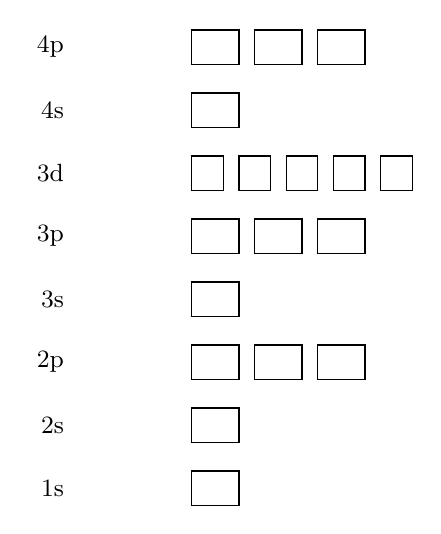
\begin{tikzpicture}[font=\small]
  \def\xlab{-1.3}
  \coordinate (y1) at (0,0);   % 1s
  \coordinate (y2) at (0,0.8); % 2s
  \coordinate (y3) at (0,1.6); % 2p
  \coordinate (y4) at (0,2.4); % 3s
  \coordinate (y5) at (0,3.2); % 3p
  \coordinate (y6) at (0,4.0); % 3d (five)
  \coordinate (y7) at (0,4.8); % 4s
  \coordinate (y8) at (0,5.6); % 4p (three)

  % 1s
  \node[left] at ($(y1)+(\xlab,0)$){1s};
  \draw ($(y1)+(0.2,-0.22)$) rectangle ($(y1)+(0.8,0.22)$);

  % 2s
  \node[left] at ($(y2)+(\xlab,0)$){2s};
  \draw ($(y2)+(0.2,-0.22)$) rectangle ($(y2)+(0.8,0.22)$);

  % 2p
  \node[left] at ($(y3)+(\xlab,0)$){2p};
  \foreach \i in {0,1,2}{
    \draw ($(y3)+(0.2+0.8*\i,-0.22)$) rectangle ($(y3)+(0.8+0.8*\i,0.22)$);
  }

  % 3s
  \node[left] at ($(y4)+(\xlab,0)$){3s};
  \draw ($(y4)+(0.2,-0.22)$) rectangle ($(y4)+(0.8,0.22)$);

  % 3p
  \node[left] at ($(y5)+(\xlab,0)$){3p};
  \foreach \i in {0,1,2}{
    \draw ($(y5)+(0.2+0.8*\i,-0.22)$) rectangle ($(y5)+(0.8+0.8*\i,0.22)$);
  }

  % 3d
  \node[left] at ($(y6)+(\xlab,0)$){3d};
  \foreach \i in {0,1,2,3,4}{
    \draw ($(y6)+(0.2+0.6*\i,-0.22)$) rectangle ($(y6)+(0.6+0.6*\i,0.22)$);
  }

  % 4s
  \node[left] at ($(y7)+(\xlab,0)$){4s};
  \draw ($(y7)+(0.2,-0.22)$) rectangle ($(y7)+(0.8,0.22)$);

  % 4p
  \node[left] at ($(y8)+(\xlab,0)$){4p};
  \foreach \i in {0,1,2}{
    \draw ($(y8)+(0.2+0.8*\i,-0.22)$) rectangle ($(y8)+(0.8+0.8*\i,0.22)$);
  }
\end{tikzpicture}
\end{minipage}
\\
\hline
\end{tabular}

\newpage
\noindent \begin{tabular}{|p{0.9\linewidth}|}
\hline
\vspace{0.2cm}
\textbf{(95)} Draw the electron diagram (orbital boxes) for neutral neon (Ne). Place arrows (↑, ↓) to indicate electrons.
\vspace{0.2cm}

\textbf{Electron configuration diagram} \\
\begin{minipage}{\linewidth}
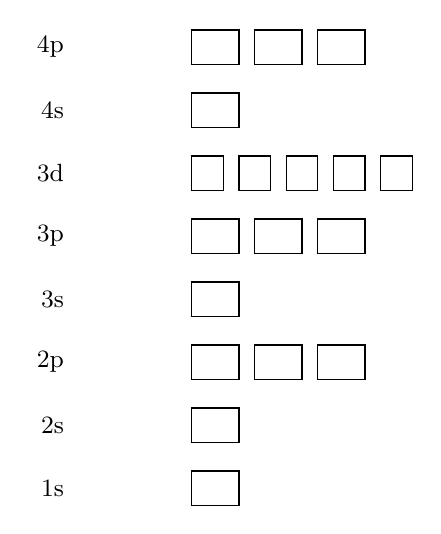
\begin{tikzpicture}[font=\small]
  \def\xlab{-1.3}
  \coordinate (y1) at (0,0);   % 1s
  \coordinate (y2) at (0,0.8); % 2s
  \coordinate (y3) at (0,1.6); % 2p
  \coordinate (y4) at (0,2.4); % 3s
  \coordinate (y5) at (0,3.2); % 3p
  \coordinate (y6) at (0,4.0); % 3d (five)
  \coordinate (y7) at (0,4.8); % 4s
  \coordinate (y8) at (0,5.6); % 4p (three)

  % 1s
  \node[left] at ($(y1)+(\xlab,0)$){1s};
  \draw ($(y1)+(0.2,-0.22)$) rectangle ($(y1)+(0.8,0.22)$);

  % 2s
  \node[left] at ($(y2)+(\xlab,0)$){2s};
  \draw ($(y2)+(0.2,-0.22)$) rectangle ($(y2)+(0.8,0.22)$);

  % 2p
  \node[left] at ($(y3)+(\xlab,0)$){2p};
  \foreach \i in {0,1,2}{
    \draw ($(y3)+(0.2+0.8*\i,-0.22)$) rectangle ($(y3)+(0.8+0.8*\i,0.22)$);
  }

  % 3s
  \node[left] at ($(y4)+(\xlab,0)$){3s};
  \draw ($(y4)+(0.2,-0.22)$) rectangle ($(y4)+(0.8,0.22)$);

  % 3p
  \node[left] at ($(y5)+(\xlab,0)$){3p};
  \foreach \i in {0,1,2}{
    \draw ($(y5)+(0.2+0.8*\i,-0.22)$) rectangle ($(y5)+(0.8+0.8*\i,0.22)$);
  }

  % 3d
  \node[left] at ($(y6)+(\xlab,0)$){3d};
  \foreach \i in {0,1,2,3,4}{
    \draw ($(y6)+(0.2+0.6*\i,-0.22)$) rectangle ($(y6)+(0.6+0.6*\i,0.22)$);
  }

  % 4s
  \node[left] at ($(y7)+(\xlab,0)$){4s};
  \draw ($(y7)+(0.2,-0.22)$) rectangle ($(y7)+(0.8,0.22)$);

  % 4p
  \node[left] at ($(y8)+(\xlab,0)$){4p};
  \foreach \i in {0,1,2}{
    \draw ($(y8)+(0.2+0.8*\i,-0.22)$) rectangle ($(y8)+(0.8+0.8*\i,0.22)$);
  }
\end{tikzpicture}
\end{minipage}
\\
\hline
\end{tabular}

\newpage
\noindent \begin{tabular}{|p{0.9\linewidth}|}
\hline
\vspace{0.2cm}
\textbf{(96)} Draw the electron diagram (orbital boxes) for neutral magnesium (Mg). Place arrows (↑, ↓) to indicate electrons.
\vspace{0.2cm}

\textbf{Electron configuration diagram} \\
\begin{minipage}{\linewidth}
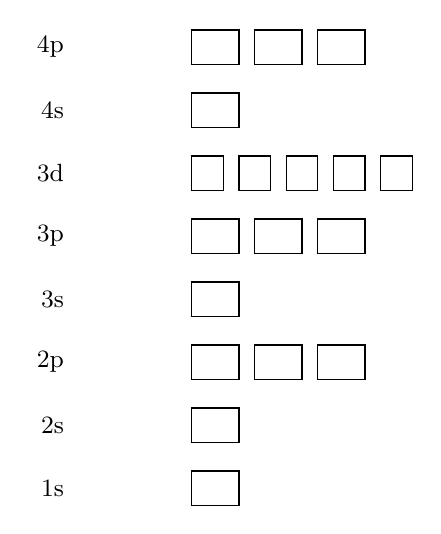
\begin{tikzpicture}[font=\small]
  \def\xlab{-1.3}
  \coordinate (y1) at (0,0);   % 1s
  \coordinate (y2) at (0,0.8); % 2s
  \coordinate (y3) at (0,1.6); % 2p
  \coordinate (y4) at (0,2.4); % 3s
  \coordinate (y5) at (0,3.2); % 3p
  \coordinate (y6) at (0,4.0); % 3d (five)
  \coordinate (y7) at (0,4.8); % 4s
  \coordinate (y8) at (0,5.6); % 4p (three)

  % 1s
  \node[left] at ($(y1)+(\xlab,0)$){1s};
  \draw ($(y1)+(0.2,-0.22)$) rectangle ($(y1)+(0.8,0.22)$);

  % 2s
  \node[left] at ($(y2)+(\xlab,0)$){2s};
  \draw ($(y2)+(0.2,-0.22)$) rectangle ($(y2)+(0.8,0.22)$);

  % 2p
  \node[left] at ($(y3)+(\xlab,0)$){2p};
  \foreach \i in {0,1,2}{
    \draw ($(y3)+(0.2+0.8*\i,-0.22)$) rectangle ($(y3)+(0.8+0.8*\i,0.22)$);
  }

  % 3s
  \node[left] at ($(y4)+(\xlab,0)$){3s};
  \draw ($(y4)+(0.2,-0.22)$) rectangle ($(y4)+(0.8,0.22)$);

  % 3p
  \node[left] at ($(y5)+(\xlab,0)$){3p};
  \foreach \i in {0,1,2}{
    \draw ($(y5)+(0.2+0.8*\i,-0.22)$) rectangle ($(y5)+(0.8+0.8*\i,0.22)$);
  }

  % 3d
  \node[left] at ($(y6)+(\xlab,0)$){3d};
  \foreach \i in {0,1,2,3,4}{
    \draw ($(y6)+(0.2+0.6*\i,-0.22)$) rectangle ($(y6)+(0.6+0.6*\i,0.22)$);
  }

  % 4s
  \node[left] at ($(y7)+(\xlab,0)$){4s};
  \draw ($(y7)+(0.2,-0.22)$) rectangle ($(y7)+(0.8,0.22)$);

  % 4p
  \node[left] at ($(y8)+(\xlab,0)$){4p};
  \foreach \i in {0,1,2}{
    \draw ($(y8)+(0.2+0.8*\i,-0.22)$) rectangle ($(y8)+(0.8+0.8*\i,0.22)$);
  }
\end{tikzpicture}
\end{minipage}
\\
\hline
\end{tabular}

\newpage
\noindent \begin{tabular}{|p{0.9\linewidth}|}
\hline
\vspace{0.2cm}
\textbf{(97)} Draw the electron diagram (orbital boxes) for neutral phosphorus (P). Place arrows (↑, ↓) to indicate electrons.
\vspace{0.2cm}

\textbf{Electron configuration diagram} \\
\begin{minipage}{\linewidth}
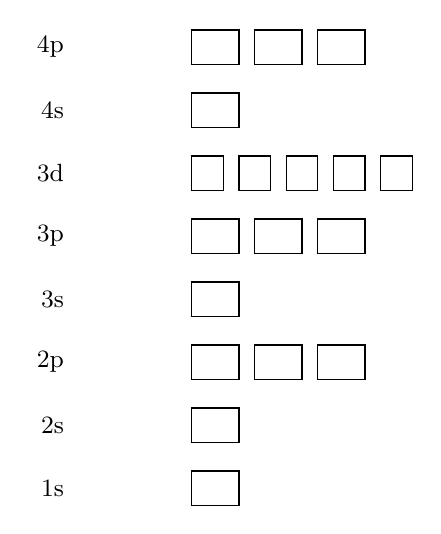
\begin{tikzpicture}[font=\small]
  \def\xlab{-1.3}
  \coordinate (y1) at (0,0);   % 1s
  \coordinate (y2) at (0,0.8); % 2s
  \coordinate (y3) at (0,1.6); % 2p
  \coordinate (y4) at (0,2.4); % 3s
  \coordinate (y5) at (0,3.2); % 3p
  \coordinate (y6) at (0,4.0); % 3d (five)
  \coordinate (y7) at (0,4.8); % 4s
  \coordinate (y8) at (0,5.6); % 4p (three)

  % 1s
  \node[left] at ($(y1)+(\xlab,0)$){1s};
  \draw ($(y1)+(0.2,-0.22)$) rectangle ($(y1)+(0.8,0.22)$);

  % 2s
  \node[left] at ($(y2)+(\xlab,0)$){2s};
  \draw ($(y2)+(0.2,-0.22)$) rectangle ($(y2)+(0.8,0.22)$);

  % 2p
  \node[left] at ($(y3)+(\xlab,0)$){2p};
  \foreach \i in {0,1,2}{
    \draw ($(y3)+(0.2+0.8*\i,-0.22)$) rectangle ($(y3)+(0.8+0.8*\i,0.22)$);
  }

  % 3s
  \node[left] at ($(y4)+(\xlab,0)$){3s};
  \draw ($(y4)+(0.2,-0.22)$) rectangle ($(y4)+(0.8,0.22)$);

  % 3p
  \node[left] at ($(y5)+(\xlab,0)$){3p};
  \foreach \i in {0,1,2}{
    \draw ($(y5)+(0.2+0.8*\i,-0.22)$) rectangle ($(y5)+(0.8+0.8*\i,0.22)$);
  }

  % 3d
  \node[left] at ($(y6)+(\xlab,0)$){3d};
  \foreach \i in {0,1,2,3,4}{
    \draw ($(y6)+(0.2+0.6*\i,-0.22)$) rectangle ($(y6)+(0.6+0.6*\i,0.22)$);
  }

  % 4s
  \node[left] at ($(y7)+(\xlab,0)$){4s};
  \draw ($(y7)+(0.2,-0.22)$) rectangle ($(y7)+(0.8,0.22)$);

  % 4p
  \node[left] at ($(y8)+(\xlab,0)$){4p};
  \foreach \i in {0,1,2}{
    \draw ($(y8)+(0.2+0.8*\i,-0.22)$) rectangle ($(y8)+(0.8+0.8*\i,0.22)$);
  }
\end{tikzpicture}
\end{minipage}
% diagram here
\\
\hline
\end{tabular}

\newpage
\noindent \begin{tabular}{|p{0.9\linewidth}|}
\hline
\vspace{0.2cm}
\textbf{(98)} Draw the electron diagram (orbital boxes) for neutral sulfur (S). Place arrows (↑, ↓) to indicate electrons.
\vspace{0.2cm}

\textbf{Electron configuration diagram} \\
\begin{minipage}{\linewidth}
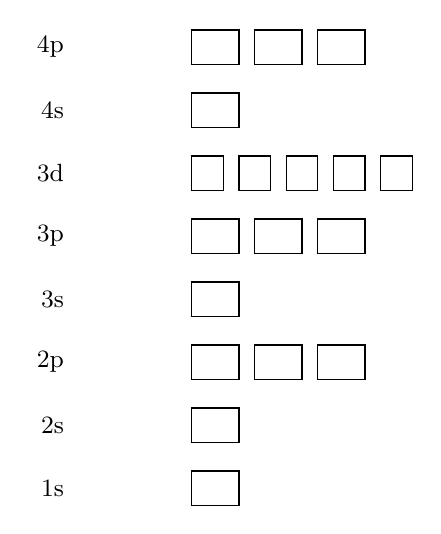
\begin{tikzpicture}[font=\small]
  \def\xlab{-1.3}
  \coordinate (y1) at (0,0);   % 1s
  \coordinate (y2) at (0,0.8); % 2s
  \coordinate (y3) at (0,1.6); % 2p
  \coordinate (y4) at (0,2.4); % 3s
  \coordinate (y5) at (0,3.2); % 3p
  \coordinate (y6) at (0,4.0); % 3d (five)
  \coordinate (y7) at (0,4.8); % 4s
  \coordinate (y8) at (0,5.6); % 4p (three)

  % 1s
  \node[left] at ($(y1)+(\xlab,0)$){1s};
  \draw ($(y1)+(0.2,-0.22)$) rectangle ($(y1)+(0.8,0.22)$);

  % 2s
  \node[left] at ($(y2)+(\xlab,0)$){2s};
  \draw ($(y2)+(0.2,-0.22)$) rectangle ($(y2)+(0.8,0.22)$);

  % 2p
  \node[left] at ($(y3)+(\xlab,0)$){2p};
  \foreach \i in {0,1,2}{
    \draw ($(y3)+(0.2+0.8*\i,-0.22)$) rectangle ($(y3)+(0.8+0.8*\i,0.22)$);
  }

  % 3s
  \node[left] at ($(y4)+(\xlab,0)$){3s};
  \draw ($(y4)+(0.2,-0.22)$) rectangle ($(y4)+(0.8,0.22)$);

  % 3p
  \node[left] at ($(y5)+(\xlab,0)$){3p};
  \foreach \i in {0,1,2}{
    \draw ($(y5)+(0.2+0.8*\i,-0.22)$) rectangle ($(y5)+(0.8+0.8*\i,0.22)$);
  }

  % 3d
  \node[left] at ($(y6)+(\xlab,0)$){3d};
  \foreach \i in {0,1,2,3,4}{
    \draw ($(y6)+(0.2+0.6*\i,-0.22)$) rectangle ($(y6)+(0.6+0.6*\i,0.22)$);
  }

  % 4s
  \node[left] at ($(y7)+(\xlab,0)$){4s};
  \draw ($(y7)+(0.2,-0.22)$) rectangle ($(y7)+(0.8,0.22)$);

  % 4p
  \node[left] at ($(y8)+(\xlab,0)$){4p};
  \foreach \i in {0,1,2}{
    \draw ($(y8)+(0.2+0.8*\i,-0.22)$) rectangle ($(y8)+(0.8+0.8*\i,0.22)$);
  }
\end{tikzpicture}
\end{minipage}
\\
\hline
\end{tabular}

\newpage
\noindent \begin{tabular}{|p{0.9\linewidth}|}
\hline
\vspace{0.2cm}
\textbf{(99)} Draw the electron diagram (orbital boxes) for neutral chlorine (Cl). Place arrows (↑, ↓) to indicate electrons.
\vspace{0.2cm}

\textbf{Electron configuration diagram} \\

\begin{minipage}{\linewidth}
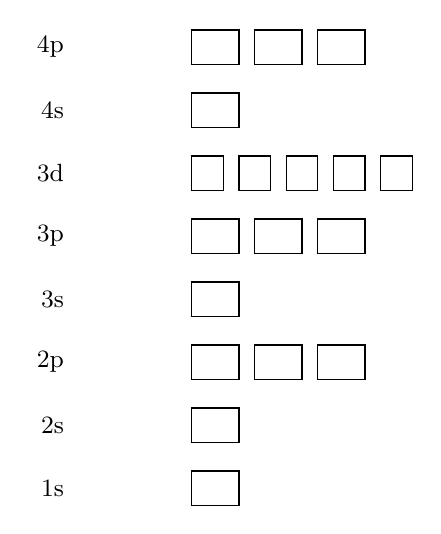
\begin{tikzpicture}[font=\small]
  \def\xlab{-1.3}
  \coordinate (y1) at (0,0);   % 1s
  \coordinate (y2) at (0,0.8); % 2s
  \coordinate (y3) at (0,1.6); % 2p
  \coordinate (y4) at (0,2.4); % 3s
  \coordinate (y5) at (0,3.2); % 3p
  \coordinate (y6) at (0,4.0); % 3d (five)
  \coordinate (y7) at (0,4.8); % 4s
  \coordinate (y8) at (0,5.6); % 4p (three)

  % 1s
  \node[left] at ($(y1)+(\xlab,0)$){1s};
  \draw ($(y1)+(0.2,-0.22)$) rectangle ($(y1)+(0.8,0.22)$);

  % 2s
  \node[left] at ($(y2)+(\xlab,0)$){2s};
  \draw ($(y2)+(0.2,-0.22)$) rectangle ($(y2)+(0.8,0.22)$);

  % 2p
  \node[left] at ($(y3)+(\xlab,0)$){2p};
  \foreach \i in {0,1,2}{
    \draw ($(y3)+(0.2+0.8*\i,-0.22)$) rectangle ($(y3)+(0.8+0.8*\i,0.22)$);
  }

  % 3s
  \node[left] at ($(y4)+(\xlab,0)$){3s};
  \draw ($(y4)+(0.2,-0.22)$) rectangle ($(y4)+(0.8,0.22)$);

  % 3p
  \node[left] at ($(y5)+(\xlab,0)$){3p};
  \foreach \i in {0,1,2}{
    \draw ($(y5)+(0.2+0.8*\i,-0.22)$) rectangle ($(y5)+(0.8+0.8*\i,0.22)$);
  }

  % 3d
  \node[left] at ($(y6)+(\xlab,0)$){3d};
  \foreach \i in {0,1,2,3,4}{
    \draw ($(y6)+(0.2+0.6*\i,-0.22)$) rectangle ($(y6)+(0.6+0.6*\i,0.22)$);
  }

  % 4s
  \node[left] at ($(y7)+(\xlab,0)$){4s};
  \draw ($(y7)+(0.2,-0.22)$) rectangle ($(y7)+(0.8,0.22)$);

  % 4p
  \node[left] at ($(y8)+(\xlab,0)$){4p};
  \foreach \i in {0,1,2}{
    \draw ($(y8)+(0.2+0.8*\i,-0.22)$) rectangle ($(y8)+(0.8+0.8*\i,0.22)$);
  }
\end{tikzpicture}
\end{minipage}
\\
\hline
\end{tabular}

\newpage
\noindent \begin{tabular}{|p{0.9\linewidth}|}
\hline
\vspace{0.2cm}
\textbf{(100)} Draw the electron diagram (orbital boxes) for neutral calcium (Ca). Place arrows (↑, ↓) to indicate electrons.
\vspace{0.2cm}

\textbf{Electron configuration diagram} \\
\begin{minipage}{\linewidth}
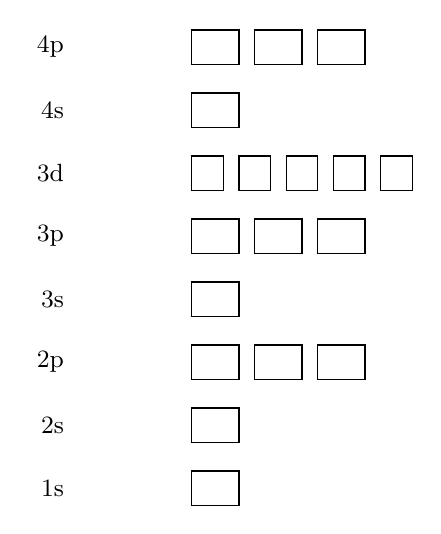
\begin{tikzpicture}[font=\small]
  \def\xlab{-1.3}
  \coordinate (y1) at (0,0);   % 1s
  \coordinate (y2) at (0,0.8); % 2s
  \coordinate (y3) at (0,1.6); % 2p
  \coordinate (y4) at (0,2.4); % 3s
  \coordinate (y5) at (0,3.2); % 3p
  \coordinate (y6) at (0,4.0); % 3d (five)
  \coordinate (y7) at (0,4.8); % 4s
  \coordinate (y8) at (0,5.6); % 4p (three)

  % 1s
  \node[left] at ($(y1)+(\xlab,0)$){1s};
  \draw ($(y1)+(0.2,-0.22)$) rectangle ($(y1)+(0.8,0.22)$);

  % 2s
  \node[left] at ($(y2)+(\xlab,0)$){2s};
  \draw ($(y2)+(0.2,-0.22)$) rectangle ($(y2)+(0.8,0.22)$);

  % 2p
  \node[left] at ($(y3)+(\xlab,0)$){2p};
  \foreach \i in {0,1,2}{
    \draw ($(y3)+(0.2+0.8*\i,-0.22)$) rectangle ($(y3)+(0.8+0.8*\i,0.22)$);
  }

  % 3s
  \node[left] at ($(y4)+(\xlab,0)$){3s};
  \draw ($(y4)+(0.2,-0.22)$) rectangle ($(y4)+(0.8,0.22)$);

  % 3p
  \node[left] at ($(y5)+(\xlab,0)$){3p};
  \foreach \i in {0,1,2}{
    \draw ($(y5)+(0.2+0.8*\i,-0.22)$) rectangle ($(y5)+(0.8+0.8*\i,0.22)$);
  }

  % 3d
  \node[left] at ($(y6)+(\xlab,0)$){3d};
  \foreach \i in {0,1,2,3,4}{
    \draw ($(y6)+(0.2+0.6*\i,-0.22)$) rectangle ($(y6)+(0.6+0.6*\i,0.22)$);
  }

  % 4s
  \node[left] at ($(y7)+(\xlab,0)$){4s};
  \draw ($(y7)+(0.2,-0.22)$) rectangle ($(y7)+(0.8,0.22)$);

  % 4p
  \node[left] at ($(y8)+(\xlab,0)$){4p};
  \foreach \i in {0,1,2}{
    \draw ($(y8)+(0.2+0.8*\i,-0.22)$) rectangle ($(y8)+(0.8+0.8*\i,0.22)$);
  }
\end{tikzpicture} \\
\end{minipage}
\\
\hline
\end{tabular}

\newpage
\noindent \begin{tabular}{|p{0.9\linewidth}|}
\hline
\vspace{0.2cm}
\textbf{(101)} Draw the electron diagram (orbital boxes) for neutral titanium (Ti). Place arrows (↑, ↓) to indicate electrons.
\vspace{0.2cm}

\textbf{Electron configuration diagram} \\
\begin{minipage}{\linewidth}
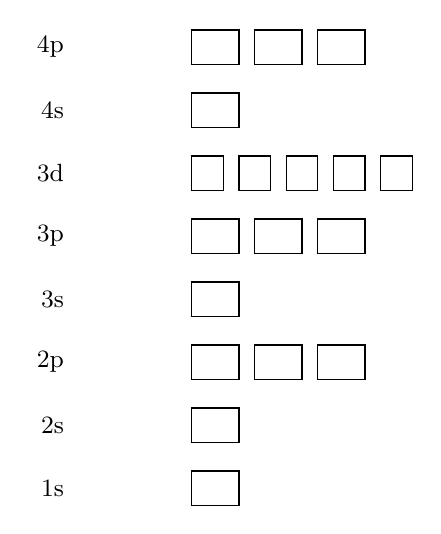
\begin{tikzpicture}[font=\small]
  \def\xlab{-1.3}
  \coordinate (y1) at (0,0);   % 1s
  \coordinate (y2) at (0,0.8); % 2s
  \coordinate (y3) at (0,1.6); % 2p
  \coordinate (y4) at (0,2.4); % 3s
  \coordinate (y5) at (0,3.2); % 3p
  \coordinate (y6) at (0,4.0); % 3d (five)
  \coordinate (y7) at (0,4.8); % 4s
  \coordinate (y8) at (0,5.6); % 4p (three)

  % 1s
  \node[left] at ($(y1)+(\xlab,0)$){1s};
  \draw ($(y1)+(0.2,-0.22)$) rectangle ($(y1)+(0.8,0.22)$);

  % 2s
  \node[left] at ($(y2)+(\xlab,0)$){2s};
  \draw ($(y2)+(0.2,-0.22)$) rectangle ($(y2)+(0.8,0.22)$);

  % 2p
  \node[left] at ($(y3)+(\xlab,0)$){2p};
  \foreach \i in {0,1,2}{
    \draw ($(y3)+(0.2+0.8*\i,-0.22)$) rectangle ($(y3)+(0.8+0.8*\i,0.22)$);
  }

  % 3s
  \node[left] at ($(y4)+(\xlab,0)$){3s};
  \draw ($(y4)+(0.2,-0.22)$) rectangle ($(y4)+(0.8,0.22)$);

  % 3p
  \node[left] at ($(y5)+(\xlab,0)$){3p};
  \foreach \i in {0,1,2}{
    \draw ($(y5)+(0.2+0.8*\i,-0.22)$) rectangle ($(y5)+(0.8+0.8*\i,0.22)$);
  }

  % 3d
  \node[left] at ($(y6)+(\xlab,0)$){3d};
  \foreach \i in {0,1,2,3,4}{
    \draw ($(y6)+(0.2+0.6*\i,-0.22)$) rectangle ($(y6)+(0.6+0.6*\i,0.22)$);
  }

  % 4s
  \node[left] at ($(y7)+(\xlab,0)$){4s};
  \draw ($(y7)+(0.2,-0.22)$) rectangle ($(y7)+(0.8,0.22)$);

  % 4p
  \node[left] at ($(y8)+(\xlab,0)$){4p};
  \foreach \i in {0,1,2}{
    \draw ($(y8)+(0.2+0.8*\i,-0.22)$) rectangle ($(y8)+(0.8+0.8*\i,0.22)$);
  }
\end{tikzpicture} \\
\end{minipage}
\\
\hline
\end{tabular}

\newpage
\noindent \begin{tabular}{|p{0.9\linewidth}|}
\hline
\vspace{0.2cm}
\textbf{(102)} Draw the electron diagram (orbital boxes) for neutral vanadium (V). Place arrows (↑, ↓) to indicate electrons.
\vspace{0.2cm}

\textbf{Electron configuration diagram} \\
\begin{minipage}{\linewidth}
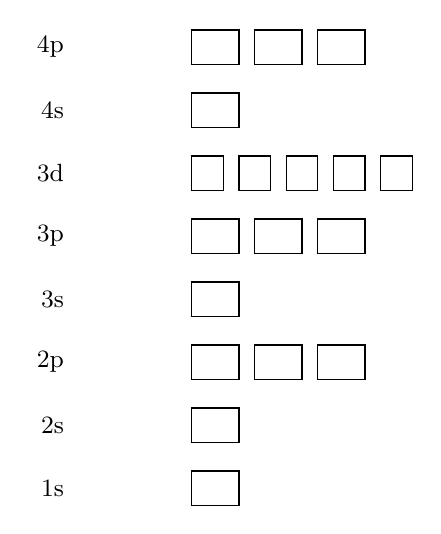
\begin{tikzpicture}[font=\small]
  \def\xlab{-1.3}
  \coordinate (y1) at (0,0);   % 1s
  \coordinate (y2) at (0,0.8); % 2s
  \coordinate (y3) at (0,1.6); % 2p
  \coordinate (y4) at (0,2.4); % 3s
  \coordinate (y5) at (0,3.2); % 3p
  \coordinate (y6) at (0,4.0); % 3d (five)
  \coordinate (y7) at (0,4.8); % 4s
  \coordinate (y8) at (0,5.6); % 4p (three)

  % 1s
  \node[left] at ($(y1)+(\xlab,0)$){1s};
  \draw ($(y1)+(0.2,-0.22)$) rectangle ($(y1)+(0.8,0.22)$);

  % 2s
  \node[left] at ($(y2)+(\xlab,0)$){2s};
  \draw ($(y2)+(0.2,-0.22)$) rectangle ($(y2)+(0.8,0.22)$);

  % 2p
  \node[left] at ($(y3)+(\xlab,0)$){2p};
  \foreach \i in {0,1,2}{
    \draw ($(y3)+(0.2+0.8*\i,-0.22)$) rectangle ($(y3)+(0.8+0.8*\i,0.22)$);
  }

  % 3s
  \node[left] at ($(y4)+(\xlab,0)$){3s};
  \draw ($(y4)+(0.2,-0.22)$) rectangle ($(y4)+(0.8,0.22)$);

  % 3p
  \node[left] at ($(y5)+(\xlab,0)$){3p};
  \foreach \i in {0,1,2}{
    \draw ($(y5)+(0.2+0.8*\i,-0.22)$) rectangle ($(y5)+(0.8+0.8*\i,0.22)$);
  }

  % 3d
  \node[left] at ($(y6)+(\xlab,0)$){3d};
  \foreach \i in {0,1,2,3,4}{
    \draw ($(y6)+(0.2+0.6*\i,-0.22)$) rectangle ($(y6)+(0.6+0.6*\i,0.22)$);
  }

  % 4s
  \node[left] at ($(y7)+(\xlab,0)$){4s};
  \draw ($(y7)+(0.2,-0.22)$) rectangle ($(y7)+(0.8,0.22)$);

  % 4p
  \node[left] at ($(y8)+(\xlab,0)$){4p};
  \foreach \i in {0,1,2}{
    \draw ($(y8)+(0.2+0.8*\i,-0.22)$) rectangle ($(y8)+(0.8+0.8*\i,0.22)$);
  }
\end{tikzpicture} \\
\end{minipage}
\\
\hline
\end{tabular}

\newpage
\noindent \begin{tabular}{|p{0.9\linewidth}|}
\hline
\vspace{0.2cm}
\textbf{(103)} Draw the electron diagram (orbital boxes) for neutral zinc (Zn). Place arrows (↑, ↓) to indicate electrons.
\vspace{0.2cm}

\textbf{Electron configuration diagram}
\vspace{0.2cm}

\textbf{Electron configuration diagram} \\
\begin{minipage}{\linewidth}
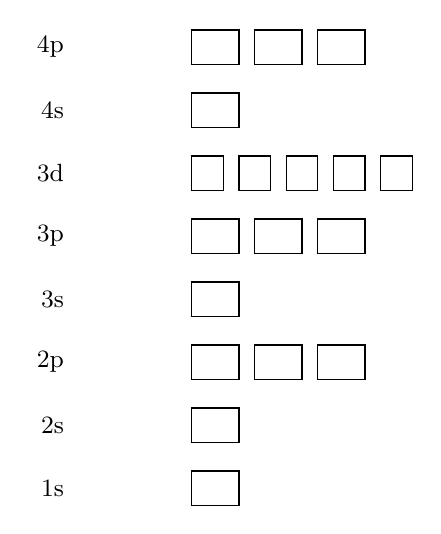
\begin{tikzpicture}[font=\small]
  \def\xlab{-1.3}
  \coordinate (y1) at (0,0);   % 1s
  \coordinate (y2) at (0,0.8); % 2s
  \coordinate (y3) at (0,1.6); % 2p
  \coordinate (y4) at (0,2.4); % 3s
  \coordinate (y5) at (0,3.2); % 3p
  \coordinate (y6) at (0,4.0); % 3d (five)
  \coordinate (y7) at (0,4.8); % 4s
  \coordinate (y8) at (0,5.6); % 4p (three)

  % 1s
  \node[left] at ($(y1)+(\xlab,0)$){1s};
  \draw ($(y1)+(0.2,-0.22)$) rectangle ($(y1)+(0.8,0.22)$);

  % 2s
  \node[left] at ($(y2)+(\xlab,0)$){2s};
  \draw ($(y2)+(0.2,-0.22)$) rectangle ($(y2)+(0.8,0.22)$);

  % 2p
  \node[left] at ($(y3)+(\xlab,0)$){2p};
  \foreach \i in {0,1,2}{
    \draw ($(y3)+(0.2+0.8*\i,-0.22)$) rectangle ($(y3)+(0.8+0.8*\i,0.22)$);
  }

  % 3s
  \node[left] at ($(y4)+(\xlab,0)$){3s};
  \draw ($(y4)+(0.2,-0.22)$) rectangle ($(y4)+(0.8,0.22)$);

  % 3p
  \node[left] at ($(y5)+(\xlab,0)$){3p};
  \foreach \i in {0,1,2}{
    \draw ($(y5)+(0.2+0.8*\i,-0.22)$) rectangle ($(y5)+(0.8+0.8*\i,0.22)$);
  }

  % 3d
  \node[left] at ($(y6)+(\xlab,0)$){3d};
  \foreach \i in {0,1,2,3,4}{
    \draw ($(y6)+(0.2+0.6*\i,-0.22)$) rectangle ($(y6)+(0.6+0.6*\i,0.22)$);
  }

  % 4s
  \node[left] at ($(y7)+(\xlab,0)$){4s};
  \draw ($(y7)+(0.2,-0.22)$) rectangle ($(y7)+(0.8,0.22)$);

  % 4p
  \node[left] at ($(y8)+(\xlab,0)$){4p};
  \foreach \i in {0,1,2}{
    \draw ($(y8)+(0.2+0.8*\i,-0.22)$) rectangle ($(y8)+(0.8+0.8*\i,0.22)$);
  }
\end{tikzpicture}\\
\end{minipage}
\\
\hline
\end{tabular}

\vspace{0.2cm}
\noindent
\begin{tabular}{|p{0.9\linewidth}|}
\hline
\vspace{0.2cm}
\textbf{(104)} What is the correct formula for the sulfate ion? \\
\begin{minipage}[t]{0.85\linewidth}
\begin{enumerate}[label=\alph*.]
\item $\text{SO}_3^{2-}$ \\
\item $\text{SO}_4^{2-}$ \\
\item $\text{SO}_4^{-}$ \\
\item $\text{SO}_3^{-}$ 
\end{enumerate}
\end{minipage}\\
\hline
\end{tabular}

\vspace{0.2cm}
\noindent
\begin{tabular}{|p{0.9\linewidth}|}
\hline
\vspace{0.2cm}
\textbf{(105)} What is the charge on the ammonium ion? \\
\begin{minipage}[t]{0.85\linewidth}
\begin{enumerate}[label=\alph*.]
\item $1-$ \\
\item $1+$ \\
\item $2+$ \\
\item $2-$
\end{enumerate}
\end{minipage}\\
\hline
\end{tabular}

\vspace{0.2cm}
\noindent
\begin{tabular}{|p{0.9\linewidth}|}
\hline
\vspace{0.2cm}
\textbf{(106)} What is the correct formula for the phosphate ion? \\
\begin{minipage}[t]{0.85\linewidth}
\begin{enumerate}[label=\alph*.]
\item $\text{PO}_3^{3-}$ \\
\item $\text{PO}_4^{3-}$ \\
\item $\text{PO}_4^{2-}$ \\
\item $\text{PO}_3^{2-}$
\end{enumerate}
\end{minipage}\\
\hline
\end{tabular}

\vspace{0.2cm}
\noindent
\begin{tabular}{|p{0.9\linewidth}|}
\hline
\vspace{0.2cm}
\textbf{(107)} What is the correct name for $\text{Fe}^{2+}$? \\
\begin{minipage}[t]{0.85\linewidth}
\begin{enumerate}[label=\alph*.]
\item Iron(I) \\
\item Iron(II) \\
\item Iron(III) \\
\item Ferrous(III)
\end{enumerate}
\end{minipage}\\
\hline
\end{tabular}

\vspace{0.2cm}
\noindent
\begin{tabular}{|p{0.9\linewidth}|}
\hline
\vspace{0.2cm}
\textbf{(108)} What is the correct formula for the carbonate ion? \\
\begin{minipage}[t]{0.85\linewidth}
\begin{enumerate}[label=\alph*.]
\item $\text{CO}_3^{2-}$ \\
\item $\text{CO}_2^{2-}$ \\
\item $\text{CO}_3^{-}$ \\
\item $\text{CO}_2^{-}$
\end{enumerate}
\end{minipage}\\
\hline
\end{tabular}

\vspace{0.2cm}
\noindent
\begin{tabular}{|p{0.9\linewidth}|}
\hline
\vspace{0.2cm}
\textbf{(109)} What is the correct name for $\text{Cu}^{+}$? \\
\begin{minipage}[t]{0.85\linewidth}
\begin{enumerate}[label=\alph*.]
\item Copper(I) \\
\item Copper(II) \\
\item Cupric(I) \\
\item Cuprous(II)
\end{enumerate}
\end{minipage}\\
\hline
\end{tabular}

\vspace{0.2cm}
\noindent
\begin{tabular}{|p{0.9\linewidth}|}
\hline
\vspace{0.2cm}
\textbf{(110)} What is the correct formula for the hydroxide ion? \\
\begin{minipage}[t]{0.85\linewidth}
\begin{enumerate}[label=\alph*.]
\item $\text{OH}^{-}$ \\
\item $\text{OH}^{+}$ \\
\item $\text{HO}^{2-}$ \\
\item $\text{HO}^{+}$
\end{enumerate}
\end{minipage}\\
\hline
\end{tabular}

\vspace{0.2cm}
\noindent
\begin{tabular}{|p{0.9\linewidth}|}
\hline
\vspace{0.2cm}
\textbf{(111)} What is the correct name for $\text{NO}_3^{-}$? \\
\begin{minipage}[t]{0.85\linewidth}
\begin{enumerate}[label=\alph*.]
\item Nitrite \\
\item Nitrate \\
\item Nitronate \\
\item Nitronite
\end{enumerate}
\end{minipage}\\
\hline
\end{tabular}

\vspace{0.2cm}
\noindent
\begin{tabular}{|p{0.9\linewidth}|}
\hline
\vspace{0.2cm}
\textbf{(112)} What is the correct formula for the ammonium ion? \\
\begin{minipage}[t]{0.85\linewidth}
\begin{enumerate}[label=\alph*.]
\item $\text{NH}_4^{-}$ \\
\item $\text{NH}_3^{+}$ \\
\item $\text{NH}_4^{+}$ \\
\item $\text{NH}_3^{-}$
\end{enumerate}
\end{minipage}\\
\hline
\end{tabular}


\end{document}

\vspace{0.2cm}
\noindent
\begin{tabular}{|p{0.9\linewidth}|}
\hline
\vspace{0.2cm}
\textbf{(113)} What is the correct name for $\text{MnO}_4^{-}$? \\
\begin{minipage}[t]{0.85\linewidth}
\begin{enumerate}[label=\alph*.]
\item Manganate \\
\item Permanganate \\
\item Manganese oxide \\
\item Manganite
\end{enumerate}
\end{minipage}\\
\hline
\end{tabular}







